\begin{frame}{Settings}

\vfill

\begin{align}
B \land H \quad &\models \quad E \\
B \land \overline{E} \quad &\models \quad \overline{H} \\
B \land \overline{E} \quad &\models \quad \overline{\bot} \\
\overline{\bot} \quad &\models \quad \overline{H} \\
H \quad &\models \quad \bot
\end{align}

\vfill

\begin{multicols}{2}
\begin{itemize}
\item $B$: background knowledge
\item $H$: hypothesis
\item $E$: examples
\item $\overline{\bot}$: set of all true literals (wrt. $B \land \overline{E}$)
\item $\bot$: most specific clause
\end{itemize}
\end{multicols}

\vfill

\end{frame}


\begin{frame}{Covering algorithm}
    
\begin{algorithm}[H]
\scriptsize
\caption{Cover set algorithm}
\SetKwInOut{Input}{input}
\Input{$h,i,B,M,E$}
If $E = \emptyset$ return $B$ \\
Let $e$ be the first example in $E$ \\
Construct clause $\bot_i$ for $e$ \tcp*{Algorithm 2}
Construct clause $H$ from $\bot_i$ \tcp*{Algorithm 3}
Let $B = B \cup H$ \\
Let $E' = \{e: e \in E \text{ and } B \models e\}$ \\
Let $E = E-E'$ \\
Goto 1
\end{algorithm}

\end{frame}
% 

\begin{frame}{Algorithm for constructing $\bot_i$}

\begin{figure}
    \centering
    \textbf{Algorithm 2:} Constructing $\bot_i$ \\ \hspace{1cm} \\
    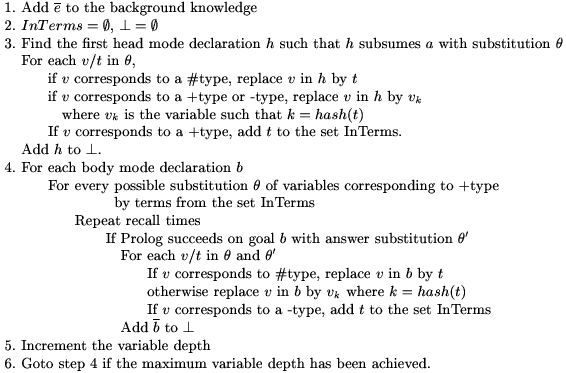
\includegraphics[scale=.5]{images/algoboti.png}\\
    \label{fig:my_label}
\end{figure}
    
\end{frame}

\begin{frame}{Algorithm for searching the lattice}

\vfill

\setcounter{algocf}{2}
\begin{algorithm}[H]
\label{algoh}
\scriptsize
\caption{Lattice search algorithm}
\SetKwInOut{Input}{input}
\Input{$h,i,B,M,E$}
$Open = \{\square\}$, $Closed = \emptyset$ \\
$s = best(Open)$, $Open = Open - s$, $Closed = Closed \cup \{s\}$  \tcp*{Node selection}
\lIf*{$prune(s)$}{goto 5  \tcp*{Node pruning}} 
$Open = (Open \cup \rho(s)) - Closed$ \tcp*{Clause refinement}
\lIf*{$terminated(Closed, Open)$}{\Return $best(Closed)$ \tcp*{End of search}}
\lIf*{$Open = \emptyset$}{\Return $e$\tcp*{No generalisation}} 
Goto 2
\end{algorithm}

\vfill

\begin{itemize}
    \item<2-> To do so, we must be able to:
    \begin{itemize}
        \item<2-> Compare solutions: $best(\cdot)$
        \item<2-> Build new hypotheses: $\rho(\cdot)$
        \item<2-> Discard wrong solutions: $prune(\cdot)$
        \item<2-> End the search: $terminated(\cdot)$
    \end{itemize}
\end{itemize}

\vfill

\end{frame}

\begin{frame}{Using numbers in the search}
\begin{multicols}{2}
\begin{itemize}
    \item $p_s$: $\#$ true positives 
    \item $n_s$: $\#$ false positives
    \item $c_s$: $\#$ atoms in body
    \item $h_s$: $\#$ optimistic estimate of literals needed
    \item $g_s = p_s-c_s-h_s$
    \item $f_s=p_s-n_s-c_s-h_s$
\end{itemize}
\end{multicols}    
\begin{itemize}
    \item $best(Open)$: returns state $s$ in set $Open$ 
    \begin{itemize}
        \item $c_s \leq c$
        \item with maximum $f_s$
    \end{itemize}
    \item $prune(s)$: returns $true$ iff either:
    \begin{itemize}
        \item $n_s=0$ and $f_s>0$
        \item $g_s \leq 0$
        \item $c_s > c$
    \end{itemize}
    \item $terminated(Closed, Open)$: return $true$ iff:
    \begin{itemize}
        \item $s = best(Closed)$, $n_s=0$, $f_s > 0$
        \item $f_s \geq g_{best(Open)}$
    \end{itemize}
\end{itemize}
\end{frame}

\begin{frame}{Learning with only positive examples}

\begin{itemize}
    \item Progol is able to learn from only positive examples
    \begin{itemize}
        \item $n_s$, in the previous slide, would always be 0
        \item An empty hypothesis would maximize $f_s$
    \end{itemize}
    \item It searches for a good compromise between the size of an hypothesis and its generality
    \item Using probability distributions, it considers the hypothesis maximizing its log-probability:
    $$ \log(P(H|E)) = d_m - m \log(g(H)) - sz(H)$$
    \item Work is still necessary to better understand how to compute the generality $g(H)$ and size $sz(H)$ of an hypothesis
\end{itemize}
    
\end{frame}
% 

\begin{frame}{Refinement operator $\rho(\cdot)$}


\begin{itemize}
    \item $s_0 = \langle\square, \emptyset, 0\rangle$
    \item $\langle C', \theta', k'\rangle \in \rho(\langle C, \theta, k\rangle)$ iff either
    \begin{enumerate}
        \item $C'=C, \, k'=k+1, \, \theta' = \theta$ ($k<n$)
        \item $C'=C\cup\{l\}, \, k'=k, \, \langle l, \theta'\rangle \in \delta(\theta, k) \text{ and } C'\in \mathcal{L}_i(M) $
    \end{enumerate}

\end{itemize}

\begin{block}{Splittable variable}
A variable is splittable if it corresponds to a +type, -type in a modeh or a -type in a modeb.
\end{block}

\begin{block}{$\langle l, \theta'\rangle \in \delta(\theta, k)$}
Let $l_k = p(u_1, \dots, u_m)$ \hfill k-th literal of $\bot_i$ \\
Let $l = p(v_1, \dots, v_m)$ \\
\begin{itemize}
    \item If $u_j$ is not splittable: $v_j/u_j \in \theta$
    \item If $u_j$ is splittable, either:
    \begin{itemize}
        \item $v_j/u_j \in \theta'$
        \item $v_j \notin dom(\theta)$, a new variable, and $\theta' = \theta\cup\{v_j/u_j\}$
    \end{itemize}
\end{itemize}

\end{block}
    
\end{frame}